\documentclass[14pt]{article}
\usepackage[a4paper,margin=2.5cm]{geometry}
\usepackage[utf8]{inputenc}
\usepackage[T1]{fontenc}
\usepackage[french]{babel}

\usepackage{graphicx}
\usepackage{xcolor}
\usepackage{fancyhdr}
\usepackage{lmodern}
\usepackage{setspace}
\usepackage{amsmath, amssymb}
\usepackage{siunitx}
\usepackage{physics}
\usepackage{hyperref}

\onehalfspacing
\pagestyle{fancy}
\fancyhf{}
\lhead{Physique}
\rhead{LHC}
\cfoot{\thepage}

\title{Une particule dans le LHC}
\author{}

\begin{document}

\maketitle
\tableofcontents

\section*{Prés requis}

\begin{enumerate}
    \item Avoir déjà entendu parlé de systèmes de coordonnées
    \item Savoir que la vitesse et l'accélération sont des vecteurs en mécanique newtonienne.
    \item Savoir faire du calcul littéral.
\end{enumerate}

\section{Etude de la trajectoire}


\subsection{Mécanique}\label{meca}

\subsubsection{Système de coordonnées}\label{coords}

Dans le contexte du LHC, les particules (protons) se déplacent dans un anneau de très grand rayon. Pour décrire leur mouvement, il est particulièrement pertinent d'utiliser un système de coordonnées cylindriques $(\rho,\varphi,z)$, adapté à la symétrie circulaire de l'accélérateur. Cela permet de distinguer facilement la position radiale (distance au centre de l'anneau), l'angle parcouru (position sur l'anneau) et la position verticale.

On rappelle que pour définir ces coordonnées, une base est nécessaire pour faire la liaison entre les coordonnées et la géométrie. Dans le cas du système de coordonnées cartésien, on utilise souvent la base canonique à l'origine du repère. La base canonique est l'ensemble des vecteurs unitaires (de norme 1) qui pointent dans les 3 directions de l'espace orthogonal entre elles (Sur la Figure - \ref{fig:cylcoords} cette base correspond aux vecteurs $\vec{u_x}$, $\vec{u_y}$, $\vec{u_z}$).

Dans les coordonnées cylindriques, on définit une base dont les directions varient en fonction de $\varphi$. Sur la Figure - \ref{fig:cylcoords}, cette base est $\vec{u_\rho}$, $\vec{u_{\varphi}}$ et $\vec{u_z}$.

Le cercle de centre $O$ et de rayon $\rho$ est très utile pour connaître les directions de la base.  
Le vecteur $\vec{u_{\rho}}$ est toujours normal (perpendiculaire) au cercle. Il part de son centre pour aller vers l'extérieur du cercle.
Le vecteur $\vec{u_{\varphi}}$ est quant à lui toujours tangent au cercle.
Pour connaître les directions de la base, on se place à un angle $\varphi$ sur le cercle et on trace les vecteurs 2 unitaires: normal vers l’extérieur et tangent dans le sens trigonométrique.

Un système que l'on veut étudier peut être représenté comme un point matériel.
Pour pouvoir repérer ce point matériel, on utilise un repère et un système de coordonnées (voir Figure - \ref{fig:cylcoords}).

On y définit les nouvelles coordonnées $\rho$, $\varphi$ et $z$ telles que:

\begin{equation} \label{eq:1.1}
    \begin{cases}
    x = \rho \cos{\varphi} \\
    y = \rho \sin{\varphi} \\
    z = z
    \end{cases}
    \tag{1.1.1}
\end{equation} 

\begin{figure}[ht]
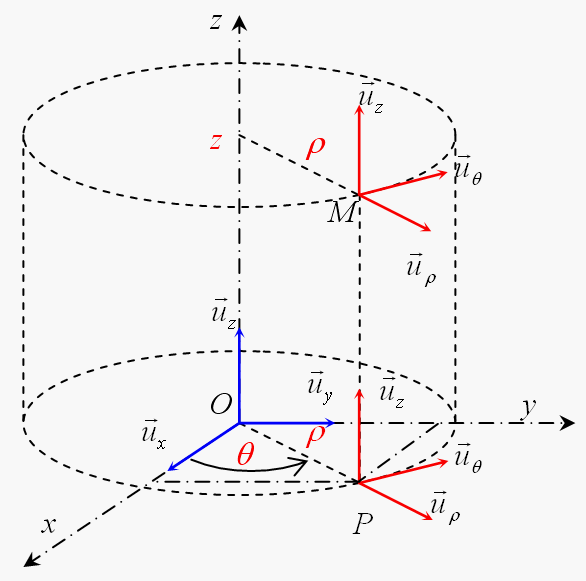
\includegraphics[width=200pt,height=200pt]{cylinder_coords.png}
\centering
\caption{
Schéma des coordonnées cylindriques\cite{henry} 
Attention à la notation, $\theta$ sur la figure correspond à $\varphi$ pour nous.
Ce schéma représente la position du point M (de coordonnée $\rho$, $\varphi$, $z$). Le point P est quand à lui la projection du point M sur le plan ($O$, $\vec{u_x}$, $\vec{u_y}$) qui est le même que le plan ($P$, $\vec{u_{\rho}}$, $\vec{u_{\varphi}}$)
}
\label{fig:cylcoords}
\end{figure}



Dans ces nouvelles coordonnées, on exprime le vecteur vitesse et le vecteur accélération comme suit:

\begin{equation}\label{eq:1.1.1a}
    \vec{v} = \dot{\rho} \vec{U_{\rho}} + \rho \dot{\varphi} \vec{U_{\varphi}}
    \tag{1.1.1a}
\end{equation}

\begin{equation}\label{eq:1.1.1b}
    \vec{a} = (\ddot{\rho} - \rho \dot{\varphi}^2) \vec{U_{\rho}} + (\rho\ddot{\varphi} + 2 \dot{\rho}\dot{\varphi}) \vec{U_{\varphi}}
    \tag{1.1.1b}
\end{equation}

\subsubsection{Principe Fondamental de la Dynamique}\label{PFD}

Le Principe Fondamental de la Dynamique (PFD) est la base de la mécanique newtonienne. Il relie la somme des forces vectorielles appliquées à un objet à son accélération. Dans un référentiel inertiel, il s'écrit :

\begin{equation} \label{eq:1.1.2}
    \sum_i \vec{F}_i = m \vec{a}
    \tag{1.1.2}
\end{equation}

Avec :
\begin{itemize}
    \item $\vec{F}_i$ : une force appliquée au système
    \item $m$ : la masse du système
    \item $\vec{a}$ : l'accélération du système
\end{itemize}

\subsubsection{Notation des dérivées temporelles}\label{deriv}

On note $\dot{x}$ la dérivée temporelle de $x$, c'est-à-dire $\dot{x} = \frac{dx}{dt}$, et $\ddot{x}$ la dérivée seconde, $\ddot{x} = \frac{d^2x}{dt^2}$.

En coordonnées cylindriques, on note $\dot{\rho}$, $\dot{\varphi}$ et $\dot{z}$ les dérivées temporelles de $\rho$, $\varphi$ et $z$ respectivement. C'est-à-dire le vecteur vitesse du point matériel dans les coordonnées cylindriques.
On note $\ddot{\rho}$, $\ddot{\varphi}$ et $\ddot{z}$ les dérivées secondes de $\rho$, $\varphi$ et $z$ respectivement. C'est-à-dire le vecteur accélération du point matériel dans les coordonnées cylindriques.


\subsubsection{Questions}

Considérons qu'un seul proton doit être accéléré pour une expérience. Avant d'être injecté dans le LHC, il est accéléré par plusieurs petits accélérateurs de particules. Une fois dans le grand tube, il continue d'être accéléré. La trajectoire souhaitée est donc circulaire et accélérée.

On pose un repère centré sur le centre du cercle formé par le tube. On utilise pour repérer le proton un système de coordonnées cylindriques.

\begin{enumerate}
    \item[Q1:] En analysant la trajectoire circulaire du proton dans le LHC, identifiez quelles coordonnées de la position ($\rho$, $\varphi$ et $z$) et de la vitesse ($\dot{\rho}$, $\dot{\varphi}$ et $\dot{z}$) restent constantes au cours du temps. Justifiez votre réponse en vous appuyant sur le mouvement.
    \item[Q2:] En déduire quelles coordonnées de l'accélération  ($\ddot{\rho}$, $\ddot{\varphi}$, $\ddot{z}$) sont nulles. En déduire la forme vectorielle simplifié de l'accélération.
    \item[Q3:] En appliquant le principe fondamental de la dynamique donner l'expression vectorielle de la force qui doit s'appliquer au proton pour qu'il suive la trajectoire circulaire imposée par le LHC? Donnez son expression en coordonnées cylindriques.
\end{enumerate}

\subsection{Champ électrique}\label{champE}

À partir de la force de Coulomb, on peut définir le champ électrique $\vec{E}$ comme étant la force par unité de charge :
\begin{equation} \label{eq:1.2}
    \vec{E} = \frac{\vec{F}}{q}
    \tag{1.2.1}
\end{equation}

Avec :
\begin{itemize}
    \item $\vec{F}$ : la force électrique
    \item $q$ : la charge du système
\end{itemize}

Cette force est analogue à la force de gravitation:

\begin{equation} \label{eq:1.2.2}
    \vec{F} = \frac{k_e q_1 q_2}{r^2} \hat{r}
    \tag{1.2.2}
\end{equation}
Avec :
\begin{itemize}
    \item $k_e$: la constante de Coulomb
    \item $q_1$ et $q_2$: les charges des deux systèmes
    \item $r$: la distance entre les deux systèmes
    \item $\hat{r}$: le vecteur unitaire qui va de $q_1$ vers $q_2$
\end{itemize}

\textit{Remarque:} Le champ électrique est conservatif, ce qui signifie que le travail effectué sur une particule ne dépend que de sa position initiale et finale.

\subsubsection{Questions}\label{q:champE}
On considère que le proton est chargé positivement et en mouvement.

Dans la réalité, le fonctionnement du LHC est extrêmement complexe avec différents types de champs magnétiques appliqués (certains pour suivre la trajectoire, d'autres pour focaliser le faisceau de protons), et un champ électrique particulier pour l'accélération (champ radiofréquence en résonance).

On simplifie le problème en considérant uniquement un champ magnétique qui permet de faire tourner le proton et un champ électrique à deux endroits du tube pour l'accélérer.


On considère que le champ électrique est appliqué à deux endroits du tube, suffisamment petits pour que l'on puisse considérer que le champ est rectiligne et constant sur ces deux portions.

\begin{enumerate}
    \item[Q4:] Dans quelle direction (vecteur de la base) doit être orienté le champ électrique dans les coordonnées cylindrique? Donner l'expression de la force électrique exercée sur le proton et discutez de son effet sur la variation d'énergie.
    \item[Q5:] En appliquant le PFD (\ref{PFD}) déterminer une des composante de l'accélération (ensemble des termes devant un vecteur de base) du proton en fonction du champ électrique $E$, de la charge du proton $q$. 
    \item[Q6:] En déduire l'expression de $\ddot{\varphi}$ en fonction de la norme de $E$ et des autres données du problèmes.
\end{enumerate}


\subsection{Champ magnétique}\label{champB}



Contrairement au champ électrique, le champ magnétique $\vec{B}$ n'est pas défini directement par une force, mais il agit sur les charges en mouvement. 
Un champ magnétique peut être généré par un courant ou par un dipôle (un aimant).

\textit{Application au LHC:} Les aimants supraconducteurs du LHC génèrent un champ magnétique intense (jusqu'à 8,3 T) pour courber la trajectoire des protons. Plus la vitesse des protons est grande, plus le champ doit être fort pour maintenir la trajectoire circulaire.


Pour un courant, la direction du champ magnétique se déduit d’une règle simple : **la règle de la main droite** (voir Figure - \ref{fig:main}).  


La règle de la main droite est très utile pour connaître la direction et le sens d'un produit vectoriel $\vec{I} \times \vec{r} = \vec{B}$.

\begin{figure}[ht]
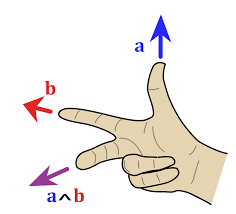
\includegraphics[width=200pt,height=200pt]{images.png}
\centering
\caption{Schéma de la règle de la main droite représentant le produit vectoriel $\vec{a} \times \vec{b}$ \cite{main}}
\label{fig:main}
\end{figure}

Voici comment l'appliquer:

\begin{itemize}
    \item Pointez le pouce de la main droite dans le sens de $\vec{a}$.
    \item Tendez l'index vers la direction de $\vec{b}$.
    \item Enfin tendez le majeur qui vous donnera la direction du résultat.
\end{itemize}


Avant de prendre quelques exemples usuels, définissons les notations des vecteurs sur les schémas.

Les vecteurs dans le plan de la feuille sont des flèches dessinées en traits pleins. Les vecteurs en traits pointillés sont derrière le plan de la feuille. Enfin, les vecteurs sortant de la feuille vers vous sont représentés par un cercle et un point au centre (comme si on voyait une flèche arriver vers nous) et les vecteurs plongeant dans la feuille sont les cercles avec une croix (comme si on voyait l'arrière de la flèche).

Il serait intéressant de verifier à l'aide de la règle de la main droite que que la direction du champ magnétique est correctement représentée par les flèches rouges sur les figures suivantes.

\textbf{Le cas d'un fil infini droit:}


On définit l'axe (Oz) suivant la direction du courant.

En utilisant la règle de la main droite, on remarque que le champ magnétique tourne autour du fil et donc de l'axe (Oz) (voir Figure - \ref{fig:fil})
 
\hspace{0.5pt}

\begin{figure}
    \centering
    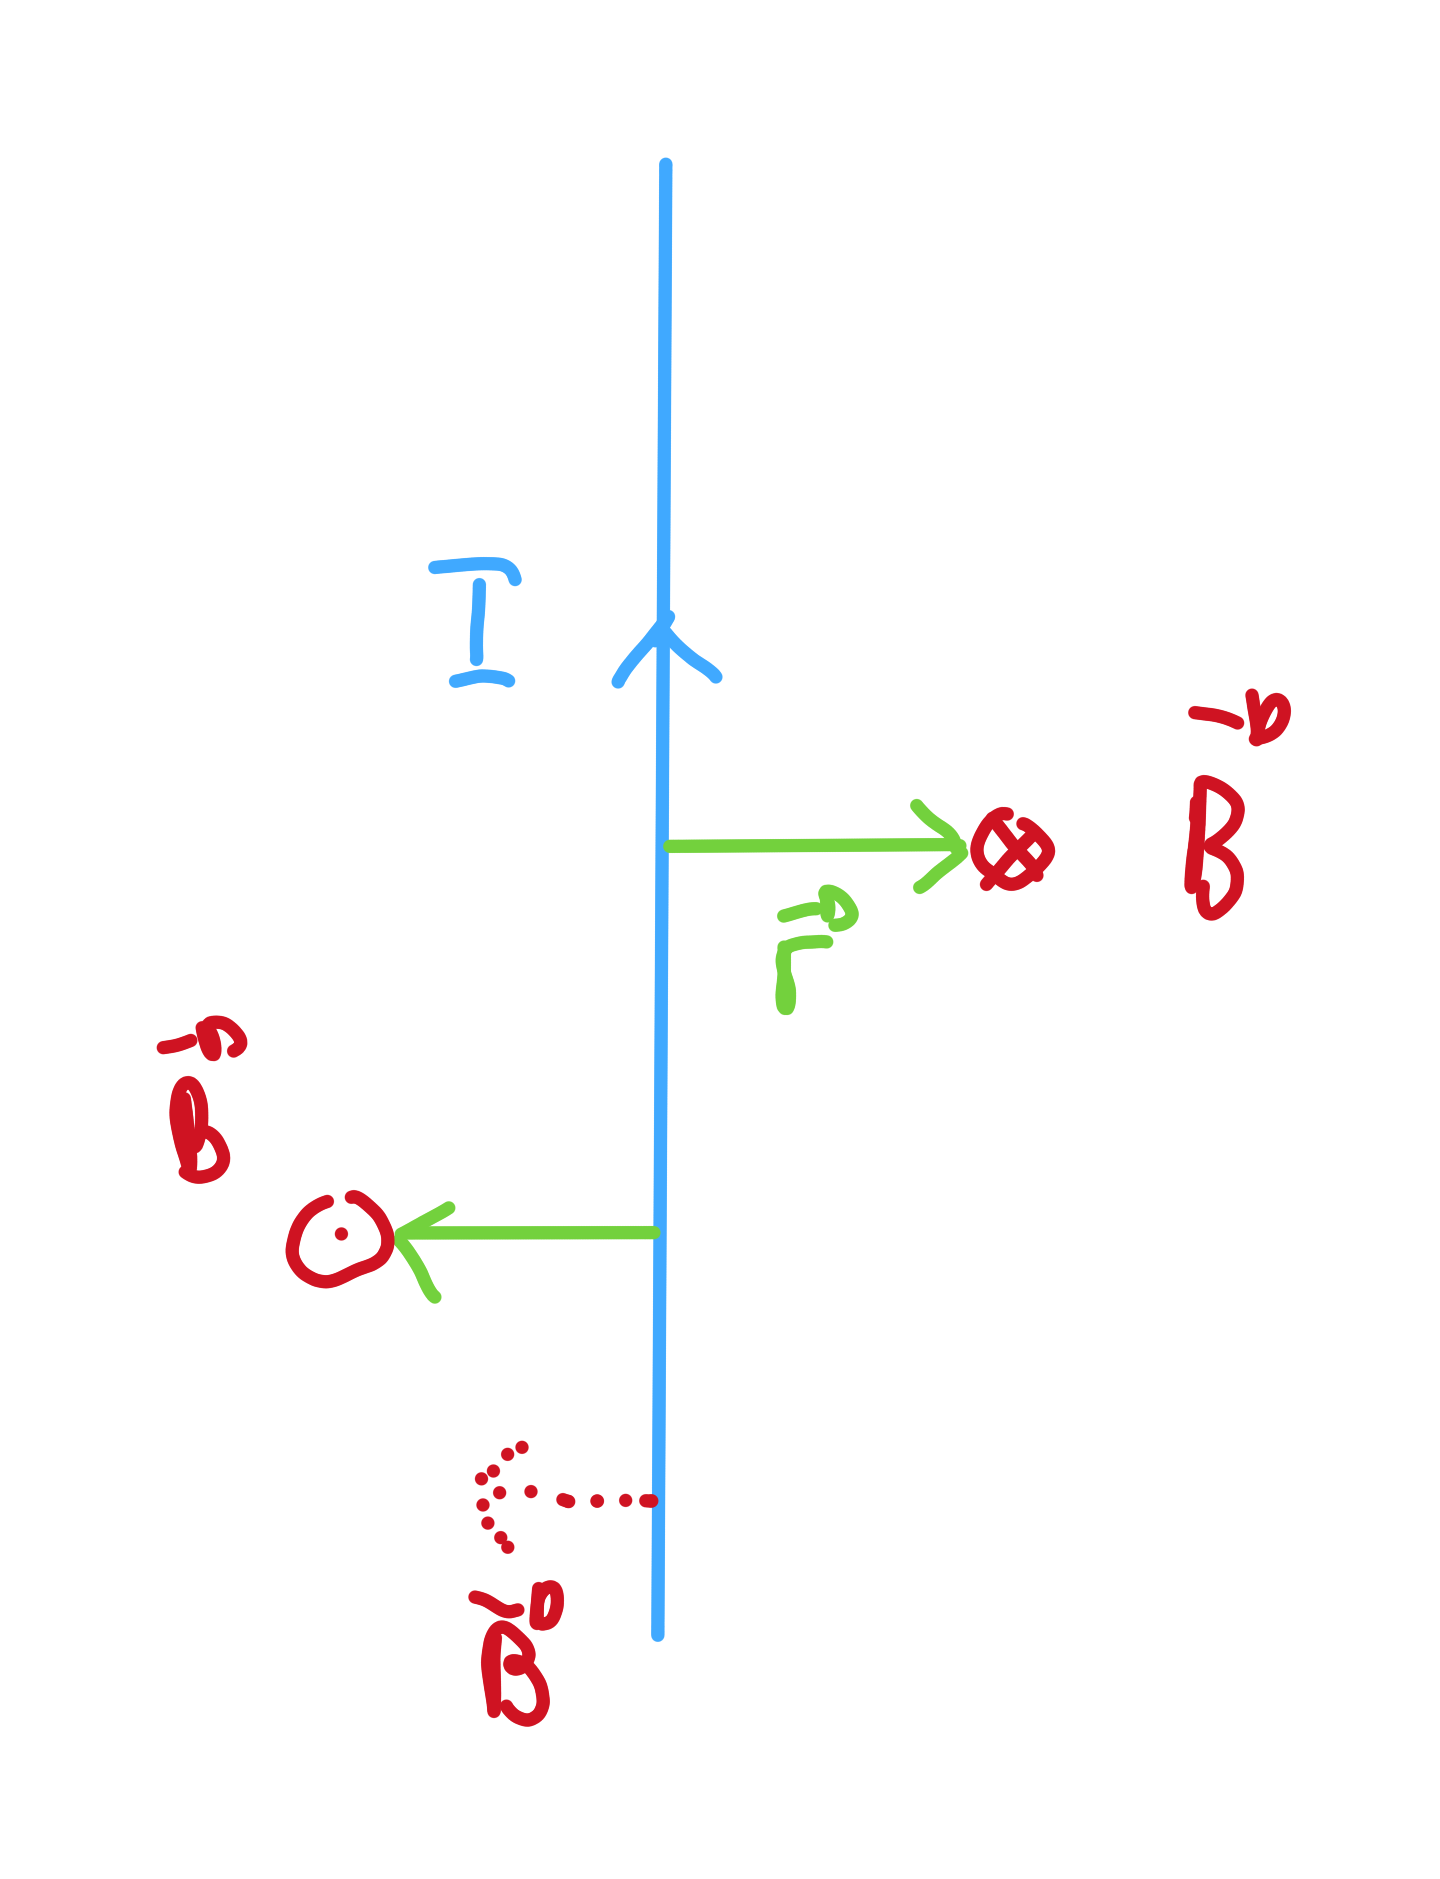
\includegraphics[width=200pt, height=200pt]{fil.png}
    \caption{Schéma du champ magnétique (en rouge) généré par un fil infini parcourus par un courant (en bleu) à la position $\vec{r}$(en vert).}
    \label{fig:fil}
\end{figure}


Pour une spire de courant, le champ magnétique au centre est :
\begin{equation} \label{eq:1.2.4}
    B = \frac{\mu_0 I}{2R}
    \tag{1.2.4}
\end{equation}

dans la direction de l'axe de la spire (voir Figure - \ref{fig:spire}).

Avec \begin{enumerate}
    \item $\mu_0$ est perméabilité magnétique du vide (une constante fondamentale)
    \item $I$ le courant circulant dans le fil
    \item R le rayon de la spire
\end{enumerate}

\begin{figure}[ht]
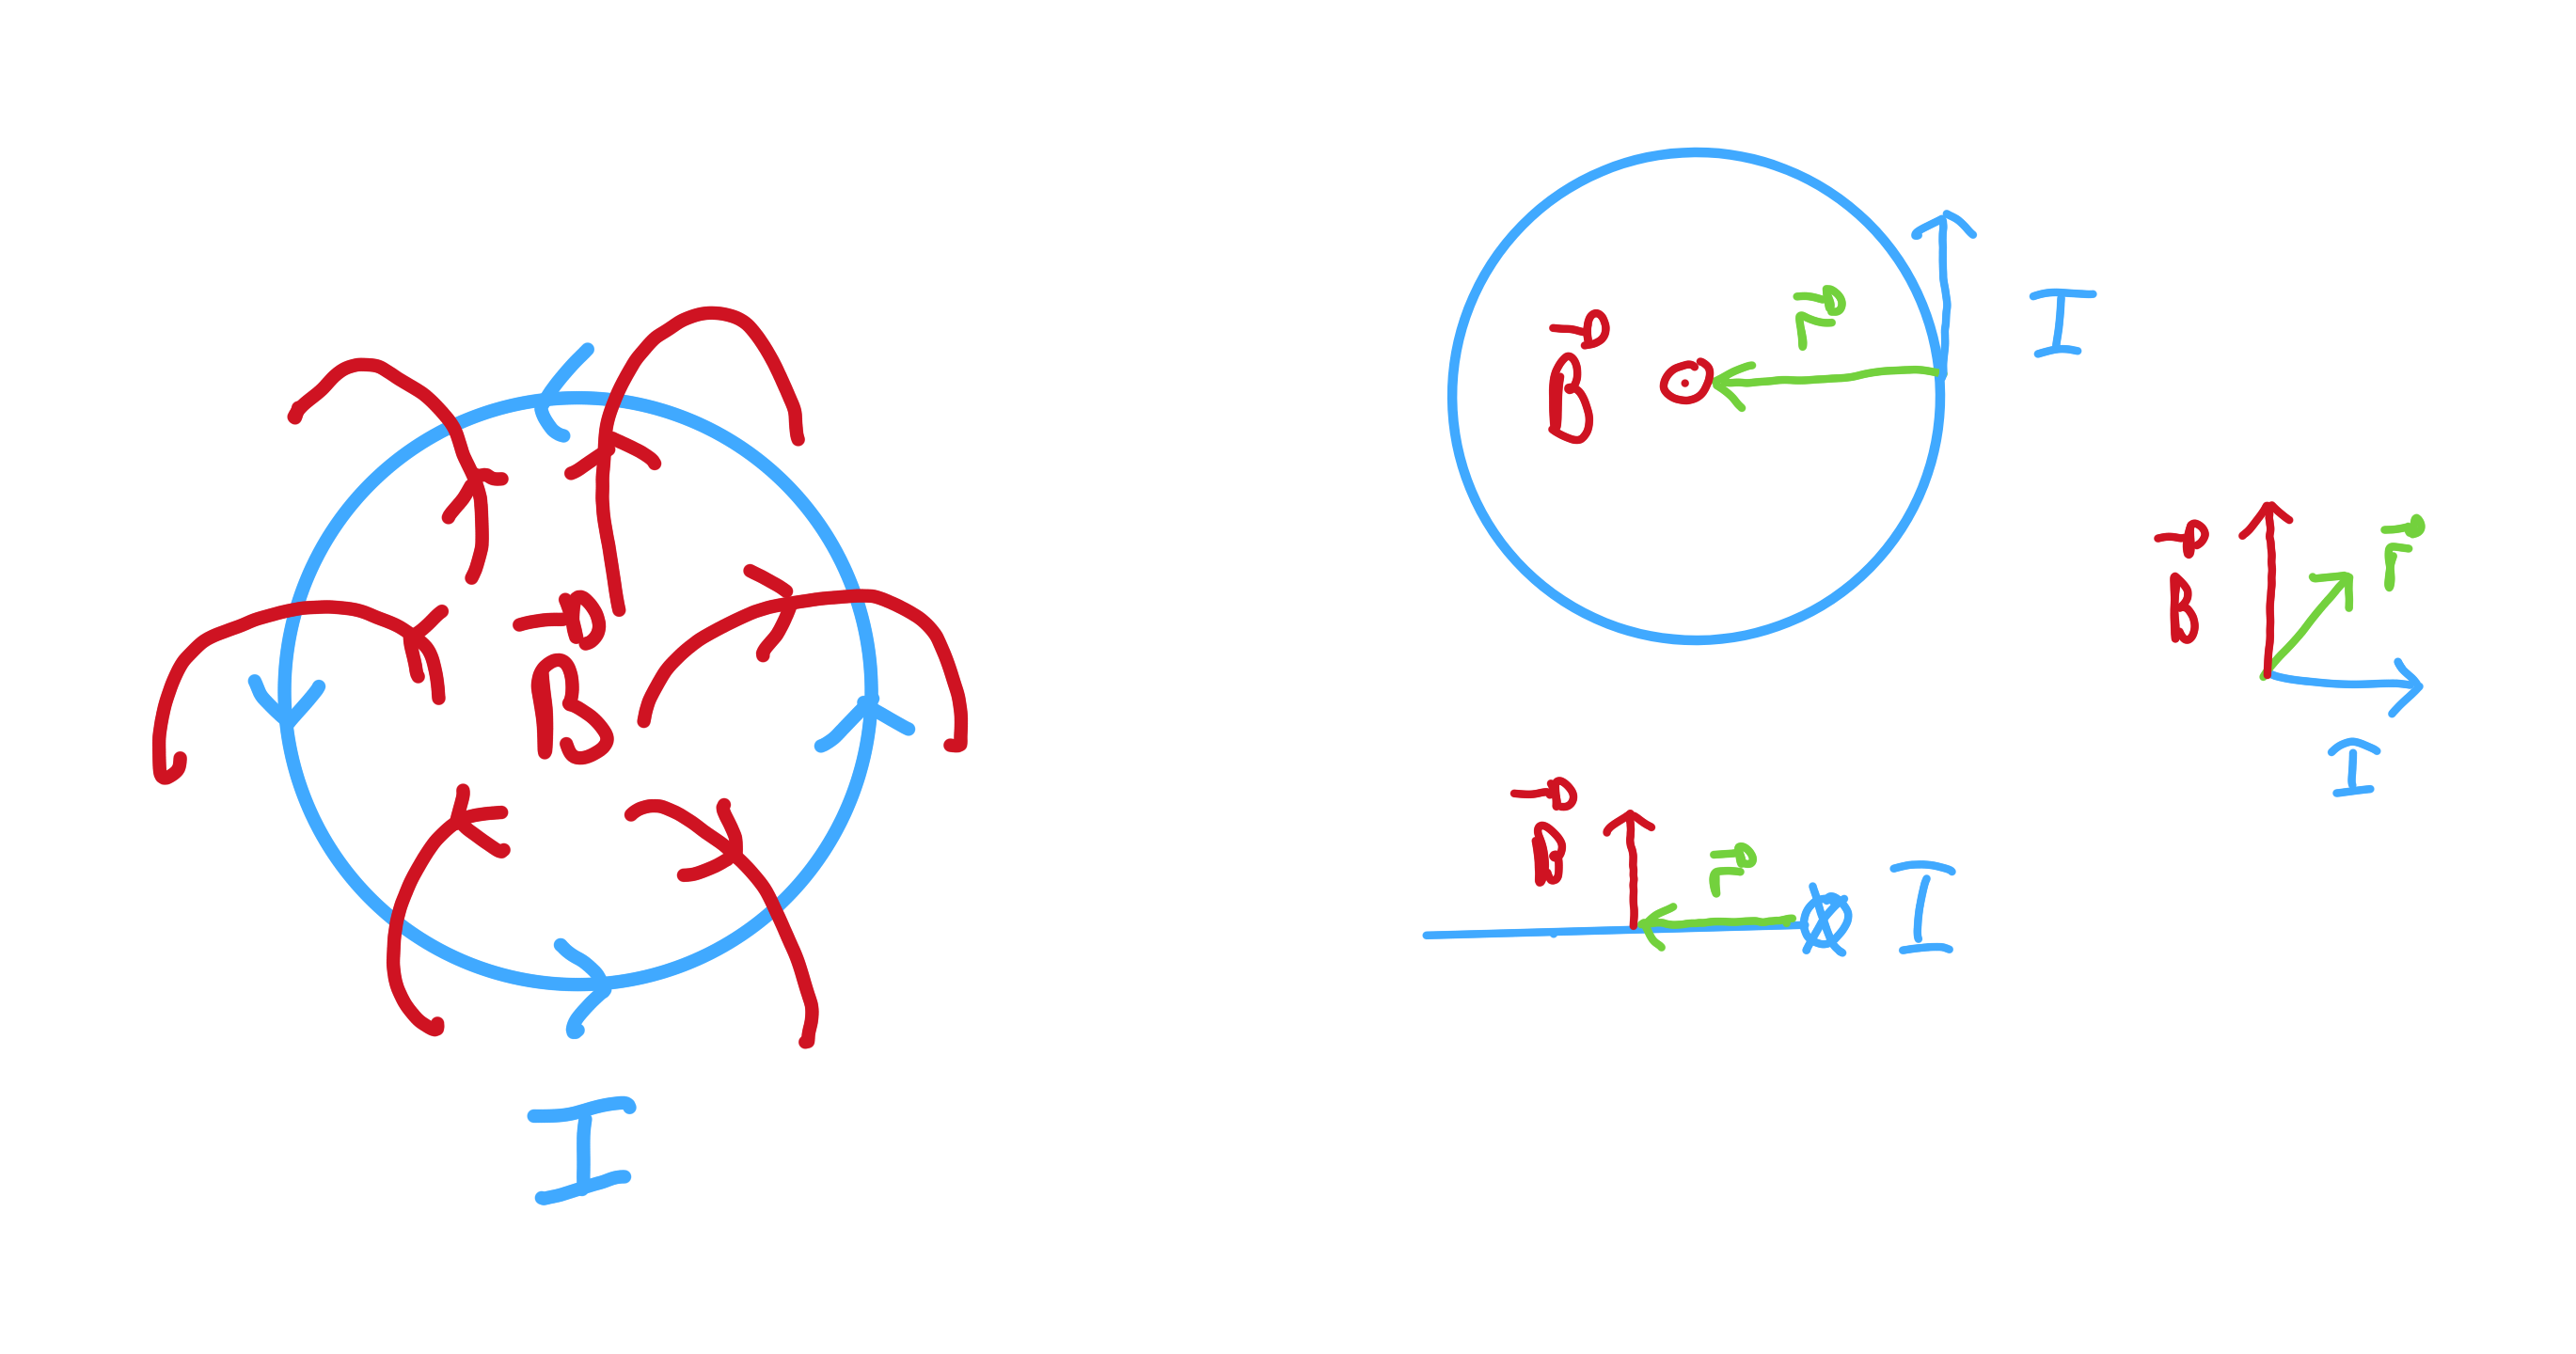
\includegraphics[width=300pt,height=200pt]{spire.png}
\centering
\caption{Schéma du champ magnétique (en rouge) généré par une spire parcourus par un courant (en bleu) à la position $\vec{r}$ (en vert).}
\label{fig:spire}
\end{figure}

\textbf{Pour une bobine infinie:}
\begin{equation} \label{eq:1.2.5}
    B = N \mu_0 I
    \tag{1.2.5}
\end{equation}

toujours dans la direction et le sens de la bobine.

On définit la force magnétique $\vec{F}$ sur une charge $q$ ayant une vitesse $\vec{v}$ dans un champ $\vec{B}$:
\begin{equation} \label{eq:1.2.6}
    \vec{F_B} = q \vec{v} \times \vec{B}
    \tag{1.2.6}
\end{equation}

\textit{Remarque:} La norme d'un produit vectoriel est le produit des normes des vecteurs.

C'est-à-dire pour la force magnétique $||\vec{F_B}|| = F_B = q v B$.



\subsubsection{Questions}\label{q:champB}
On considère que le champ magnétique est constant sur toute la trajectoire du proton. On suppose qu'il est généré par des bobines placées autour du tube.
On posera que le proton tourne dans le sens horaire dans le tube qui fait $4,5 km$ de rayon.
Pour l'application numérique, on prendra $N = 500 m^{-1}$, $m = 1.7 \times 10^{-27} kg$, $q = 1.6 \times 10^{-19} \ \ USI$, $\mu_0 = 1.3 \times 10^{-6} \ \ USI$.

\begin{enumerate}
    \item[Q7:] Quelle doit être la direction (vecteur de la base cylindrique) du champ grâce à l'aide de la règle de la main droite. Égaliser la force magnétique avec la dernière composante de l'accélération.
    \item[Q8:] En appliquant la règle de la main droite, indiquez la direction du courant autour du tube nécessaires pour générer ce champ.
    \item[Q9:] Déduisez-en l'orientation géométrique des bobines autour du tube du LHC, c'est à dire quel est l'orientation et la position de la bobine par rapport au tube. On pourra faire un schéma pour expliciter sa réponse. 
    \item[Q10:] 
    \begin{enumerate}
        \item[a)] Après avoir simplifier l'équation (\ref{eq:1.1.1a}), exprimer $\dot{\varphi}$ en fonction de la vitesse $v$ et du rayon $\rho$.
        \item[b)] Exprimer $B$ en fonction de $v$, $\rho$ et des autres données du problème.
        \item[c)] Quel courant doit passer dans les bobines (que l'on considère comme infini pour les calculs) pour que le proton suive la trajectoire circulaire à une vitesse de $0.2c$? 
    \end{enumerate}
\end{enumerate}

\section{Collision de deux protons}\label{colision}

\subsection{Relativité restreinte}\label{relat}

La relativité restreinte est indispensable pour décrire le mouvement des particules dans le LHC, car leur vitesse approche celle de la lumière. Les lois classiques de la mécanique ne sont alors plus valables.

\subsubsection{Principes de la relativité restreinte}\label{relatP}

La relativité restreinte, formulée par Einstein en 1905, repose sur deux postulats :
\begin{itemize}
    \item Les lois de la physique sont les mêmes dans tous les référentiels inertiels.
    \item La vitesse de la lumière dans le vide \textbf{c} est la même pour tous les observateurs, quel que soit leur mouvement relatif.
\end{itemize}

Conséquences majeures :
\begin{itemize}
    \item La simultanéité des événements dépend du référentiel.
    \item Les mesures de temps (dilatation du temps) et d'espace (contraction des longueurs) varient selon la vitesse de l'observateur.
    \item L'énergie et la masse deviennent liées (voir $E=mc^2$).
\end{itemize}

Par exemple, pour un observateur M en mouvement par rapport à un observateur R qui est au repos, la durée d'un événement mesurée par M sera plus courte que la durée mesurée par R. 

La transformation de Galilée, utilisée en mécanique classique, est remplacée par la transformation de Lorentz :
\begin{equation} \label{eq:2.1}
    \begin{cases}
        x' = \gamma (x - \beta c t) \\
        c t' = \gamma (c t - \beta x) \\
        y' = y \\
        z' = z
    \end{cases}
    \tag{2.1}
\end{equation}
avec $\beta = \frac{v}{c}$ et $\gamma(v) = \frac{1}{\sqrt{1 - \frac{v^2}{c^2}}}$.
\vspace{1em}

On nommera $\gamma(v)$ le facteur de Lorentz

\subsubsection{Loi de conservations}

En mécanique classique, seule l'énergie est conservée dans les cas de collisions élastiques ou inélastiques.

En revanche, en relativité, l'énergie et l'impulsion sont conservées dans les 2 types de collisions.

Concrètement, l'énergie totale des particules avant la collision est égale à l'énergie totale des particules produites après la collision.

L'énergie totale d'une particule en mécanique relativiste est donnée par:

\begin{equation} \label{eq:2.2}
    E = \gamma(v) m c^2
    \tag{2.2}
\end{equation}

où $\gamma(v)$ est le facteur de Lorentz.

On remarque que dans le référentiel propre de la particule, sa vitesse est nulle. L'expression de l'énergie se simplifie et devient l'expression célèbre $E = mc^2$ (où $m$ est la masse de la particule, $c$ est la vitesse de la lumière). C'est l'énergie de masse.

\textbf{Remarque:}

En relativité, on exprime la masse des particules en $eV/c^2$ (électron-volts par vitesse de la lumière au carré). Cela correspond à l'énergie de la particule dans son référentiel propre (donc de son point de vue) à $c^2$ près.

\subsection{Questions}

En réalité, le LHC est conçu pour faire entrer en collision deux faisceaux de protons qui tournent en sens inverse. On va donc considérer que deux protons tournent dans le tube du LHC, l'un dans le sens horaire et l'autre dans le sens antihoraire. On supposera également que les deux protons entrent en collision frontale, c'est-à-dire en face à face.

On supposera que les deux protons ont la même vitesse $v_p = 0.99c$ lors de la collision dans le référentiel du LHC. La masse du boson de Higgs est $m_H = 125 GeV / c^2$. La masse d'un proton est $m_p = 938 MeV/c^2$.

\begin{enumerate}
    \item[Q11:] En utilisant la formule relativiste de l'énergie (\ref{eq:2.2}) exprimez l'énergie de chaque proton dans le référentiel du LHC. Précisez qualitativement la différence entre énergie totale et énergie cinétique.
    \item[Q12:] Calculez l'énergie totale disponible lors de la collision des deux protons dans le référentiel du LHC.
    \item[Q13:] Discutez de la possibilité de produire un boson de Higgs lors de cette collision. Quelle est l'énergie minimal que doit avoir chacun des protons?
    \item[Q14:] Déterminez la vitesse minimale que doivent atteindre les protons pour permettre la création d'un boson de Higgs lors d'une collision frontale.
    \item[Q15:] Expliquer pourquoi même avec cette vitesse minimal, il serait impossible de détecter directement le boson de Higgs sachant que la collision s'effectue dans le vide.
    \item[Q16:] Que devient l'énergie total de la particule quand on fait tendre la vitesse de la particule vers la vitesse de la lumière? En déduire de la possibilité de l'atteindre ou non.
\end{enumerate}

\section*{Remerciment}

Je souhaiterais remercier Benoît pour ses conseils dans l'amélioration de ce travail.

% Amélioration de la bibliographie
\begin{thebibliography}{9}
\bibitem{henry}
Michel HENRY - Université du Maine Paternité
\bibitem{main}
\href{https://commons.wikimedia.org/wiki/File:Rechte-Hand-Regel.svg}{Canarrisderivative work}: Canarris, \href{https://creativecommons.org/licenses/by-sa/3.0}{CC BY-SA 3.0}, via Wikimedia Commons
\end{thebibliography}

\section{Annexe justification sur le choix de champ}

On a choisi que seul le champ électrique permet d'accélérer la particule et seul le champ magnétique permet de faire tourner la particule. Mais pourquoi?

Le théorème de l'énergie cinétique permet de répondre à cette question.

\subsection{Théorème de l'énergie cinétique}\label{theoEC}

Avant d'énoncer le théorème de l'énergie cinétique, on rappelle quelques définitions:
\begin{itemize}
    \item L'énergie cinétique $E_c$ d'un système est définie comme étant
    \begin{equation} \label{eq:3.1.1}
        E_c = \frac{1}{2} m v^2
        \tag{3.1.1}
    \end{equation}
    avec $v$ la vitesse du système et $m$ sa masse.
    \item On définit le travail $W$ comme l'énergie induite au système par la force $\vec{F}$ pendant le déplacement du point $A$ au point $B$.
    Il peut être positif (force motrice) ou négatif (force résistante).
\end{itemize}

\hspace{1mm}

Le théorème de l'énergie cinétique s'énonce alors :
\begin{equation} \label{eq:3.1.2}
    \Delta E_c = W
    \tag{3.1.2}
\end{equation}

Avec :
\begin{itemize}
    \item $\Delta E_c$ : variation de l'énergie cinétique du système
    \item $W$ : travail effectué par les forces appliquées au système
\end{itemize}

En clair, le théorème de l'énergie cinétique nous indique que si la force est motrice, l'énergie cinétique du système augmente (le système accélère), et si la force est résistante, l'énergie cinétique du système diminue (le système ralentit).

De plus, l'équation (\ref{eq:1.2.6}) nous indique que la force magnétique est toujours perpendiculaire à la vitesse de la particule. La norme de la vitesse n'augmente donc pas. La particule ne gagne pas d'énergie. On dit que la force magnétique ne travaille pas. C'est pourquoi on l'utilise pour faire tourner la particule. Le champ électrique travaille à l'inverse et permet donc de donner de l'énergie à la particule,ce qui l'accélère.


\section{Annexe formalisme des quadrivecteurs en relativité restreinte}


On remarque à partir de (\ref{eq:2.1}) qu'il n'est plus possible de traiter les coordonnées spatiales et temporelles de manière séparée.

On introduit donc le concept de quadrivecteur, qui regroupe les coordonnées spatiales et temporelles en un seul objet mathématique.

Pour unifier la description de l'espace et du temps, la relativité introduit la notion de quadrivecteur. Un quadrivecteur regroupe les coordonnées spatiales et temporelles d'un événement :
\begin{equation}\label{eq:4.1}
    \tilde{r} = \begin{pmatrix}
        ct \\
        x \\
        y \\
        z
    \end{pmatrix}
    \tag{4.1}
\end{equation}

Le produit scalaire de deux quadrivecteurs est:
\begin{equation}\label{eq:4.1.1}
    \tilde{r} \cdot \tilde{r}' = c^2 t t' - x x' - y y' - z z'
    \tag{4.1.1}
\end{equation}

\textit{Lien avec le LHC:} L'énergie et l'impulsion des protons sont décrites par le quadrivecteur impulsion, ce qui permet de calculer précisément les énergies mises en jeu lors des collisions.

On définit aussi le quadrivecteur vitesse $\tilde{U}$ et le quadrivecteur impulsion $\tilde{P}$:
\begin{equation} \label{eq:4.2}
    \tilde{U} = \frac{d\tilde{r}}{d\tau} = \begin{pmatrix}
        \gamma(u) c \\
        \gamma(u) u_x \\
        \gamma(u) u_y \\
        \gamma(u) u_z
    \end{pmatrix}
    \tag{4.2}
\end{equation}

\begin{equation}\label{eq:4.3}
    \tilde{P} = m \tilde{U} = \begin{pmatrix}
        \gamma(u) m c = \frac{E}{c}\\
        \gamma(u) m u_x = p_x\\
        \gamma(u) m u_y = p_y\\
        \gamma(u) m u_z = p_z
    \end{pmatrix}
    \tag{4.3}
\end{equation}

avec $\gamma(u)= \frac{1}{\sqrt{1-(\frac{u}{c})^2}}$

\textit{Remarque :} Le produit scalaire du quadrivecteur impulsion est invariant par transformation de Lorentz, ce qui permet de relier l'énergie, la masse et l'impulsion relativistes :
\begin{equation}\label{eq:4.3.1}
    \tilde{P}^2 = \frac{E^2}{c^2} - \vec{p}^{\ 2}
    \tag{4.3.1}
\end{equation}

Dans le référentiel propre de la particule:
\begin{equation}\label{eq:4.3.2}
    \tilde{P}^2 = m^2 c^2
    \tag{4.3.2}
\end{equation}

Ce formalisme est très utile pour étudier la cinématique et la dynamique en relativité. En effet, la grande particularité de ces quadrivecteurs est qu'ils sont tous invariants par la transformée de Lorentz. C'est-à-dire, on peut changer de référentiel sans se poser de questions avec ce formalisme. La composition des vitesses devient qu'une addition de quadrivecteurs...

\end{document}